\section{Gerência de Riscos - Até Ponto de Controle 2}

Com o desenvolvimento do projeto, do ponto de controle 1 até o ponto de controle 2 foram identificados novos riscos ao projeto. Os riscos e suas análises seguem os mesmos padrões já estabelecidos anteriormente. Para manter consistência, os IDs foram continuados das tabelas anteriores. As figuras a seguir mostram os riscos identificados.

\begin{figure}[H]
	\centering
	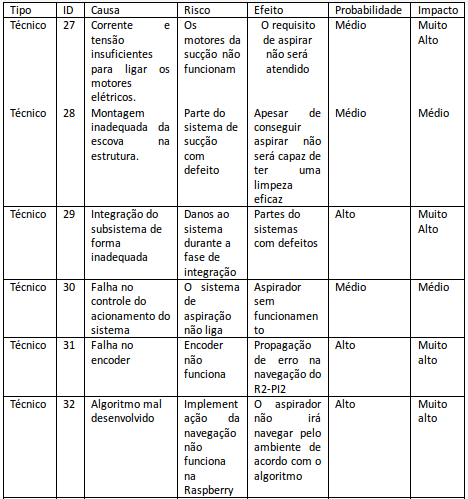
\includegraphics[scale=0.5]{figuras/riscos_pc2_1.png}
	\caption{Riscos Identificados no PC2 1.}
	\label{img:riscospc21}
\end{figure}

\begin{figure}[H]
	\centering
	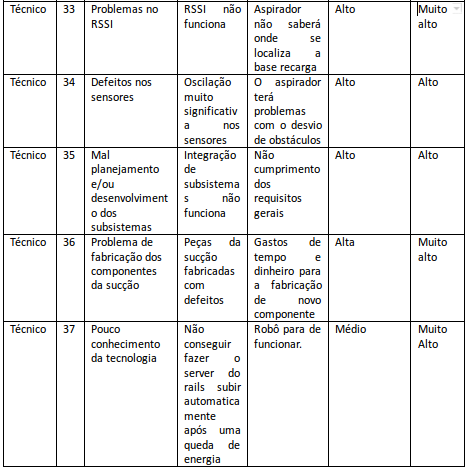
\includegraphics[scale=0.5]{figuras/riscos_pc2_2.png}
	\caption{Riscos Identificados no PC2 2.}
	\label{img:riscospc22}
\end{figure}

\begin{figure}[H]
	\centering
	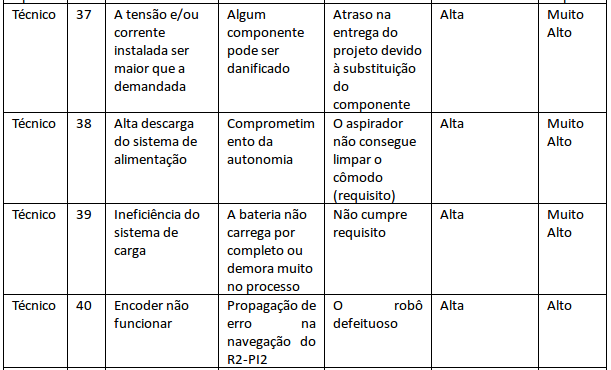
\includegraphics[scale=0.5]{figuras/riscos_pc2_3.png}
	\caption{Riscos Identificados no PC2 3.}
	\label{img:riscospc23}
\end{figure}

\begin{figure}[H]
	\centering
	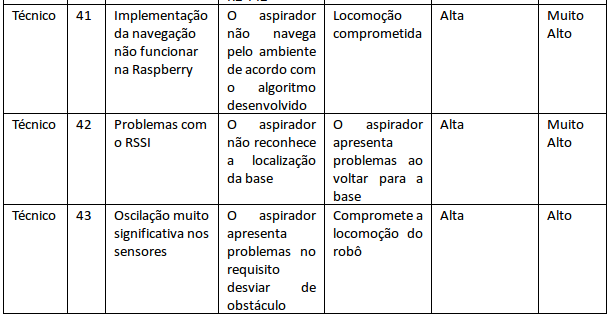
\includegraphics[scale=0.5]{figuras/riscos_pc2_4.png}
	\caption{Riscos Identificados no PC2 4.}
	\label{img:riscospc24}
\end{figure}

As figuras \ref{img:qualitativoriscospc2} e \ref{img:qualitativoriscospc22} mostra quais são as análises qualitativas dos riscos identificados.

\begin{figure}[H]
	\centering
	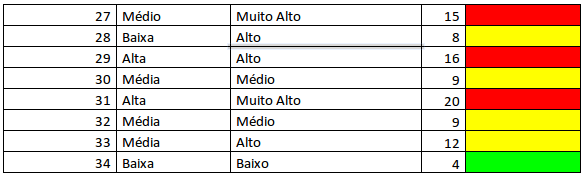
\includegraphics[scale=0.5]{figuras/riscosQualitativopc2.png}
	\caption{Qualificação dos riscos do PC2 1.}
	\label{img:qualitativoriscospc2}
\end{figure}

\begin{figure}[H]
	\centering
	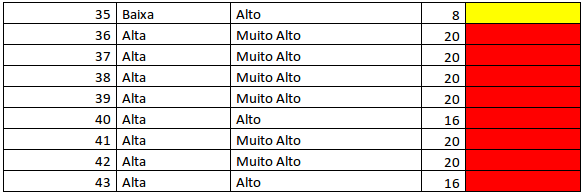
\includegraphics[scale=0.5]{figuras/riscosQualitativopc22.png}
	\caption{Qualificação dos riscos do PC2 2.}
	\label{img:qualitativoriscospc22}
\end{figure}

A seguir, as figuras mostram o plano de resposta para os novos riscos.

\begin{figure}[H]
	\centering
	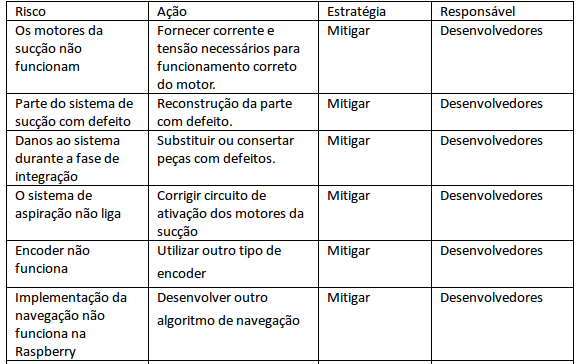
\includegraphics[scale=0.5]{figuras/riscos_acao_pc2_1.png}
	\caption{Resposta aos riscos PC2 1.}
	\label{img:respostasriscospc21}
\end{figure}

\begin{figure}[H]
	\centering
	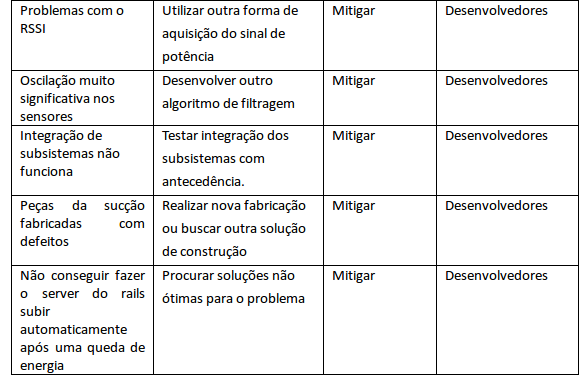
\includegraphics[scale=0.5]{figuras/riscos_acao_pc2_2.png}
	\caption{Resposta aos riscos PC2 2.}
	\label{img:respostasriscospc22}
\end{figure}

Adicionalmente, alguns dos riscos identificados ocorreram e a equipe de desenvolvimento precisou tomar ações de resposta. A tabela \ref{tab:riscosocorridos} mostra os riscos que ocorreram e quais foram as ações exatam que foram tomadas

\begin{table}[]
\centering
\caption{Riscos ocorridos e suas respostas.}
\label{tab:riscosocorridos}
\begin{tabular}{|l|l|l|}
\hline
\textbf{ID} & \textbf{Risco}                                                                                                                      & \textbf{Forma como foi solucionado}                                                                                                                      \\ \hline
3           & \begin{tabular}[c]{@{}l@{}}Sensoriamento de obstáculos \\ não funciona\end{tabular}                                                 & \begin{tabular}[c]{@{}l@{}}Trocou-se o sensor IR por sensores \\ ultrassônicos.\end{tabular}                                                             \\ \hline
11          & \begin{tabular}[c]{@{}l@{}}Vazão de ar sugado pelo \\ aspirador não é suficiente\end{tabular}                                       & \begin{tabular}[c]{@{}l@{}}Trocou-se a hélice e o motor utilizados\\ para gerar a vazão de ar suficiente\end{tabular}                                    \\ \hline
25          & \begin{tabular}[c]{@{}l@{}}Material de produção é \\ avariado\end{tabular}                                                          & \begin{tabular}[c]{@{}l@{}}Comprou-se novos materiais e em maior \\ quantidade.\end{tabular}                                                             \\ \hline
25          & \begin{tabular}[c]{@{}l@{}}Material de produção é \\ avariado\end{tabular}                                                          & \begin{tabular}[c]{@{}l@{}}Comprou-se um novo produto e se \\ modificou a estrutura para que não \\ ocorra novamente o dano ao componente\end{tabular}   \\ \hline
36          & \begin{tabular}[c]{@{}l@{}}Problemas de fabricação \\ dos componentes da sucção\end{tabular}                                        & \begin{tabular}[c]{@{}l@{}}Optou-se por comprar um modelo de \\ hélice comercial\end{tabular}                                                            \\ \hline
37          & \begin{tabular}[c]{@{}l@{}}Não conseguir fazer o server \\ do rails subir automaticamente \\ após uma queda de energia\end{tabular} & \begin{tabular}[c]{@{}l@{}}Colocou o terminal como programa \\ inicial na raspberry e no .bashrc colocou \\ para iniciar o server do rails.\end{tabular} \\ \hline
\end{tabular}
\end{table}

